\section{Lösungskonzept}
Das Lösungskonzept soll von aussen nach innen definiert werden. Darum werden zuerst die Systemgrenzen definiert. Anschliessend werden die Funktionen beschrieben. Diese werden nachfolgend in Teilsysteme unterteilt. Am Schluss wird noch ein alternativer Ansatz diskutiert, der aber nicht weiterverfolgt wird.

\subsection{Systemgrenzen}
Wie dem nachfolgendem Diagramm entnommen werden kann, wird sich das Projekt auf den Dojo konzentrieren. Alle Systeme die es für das Gesamtsystem Museum braucht, sollen nicht betrachtet werden. Die Schnittstellen werden soweit definiert, dass die Einbindung in ein Gesamtsystem keine Probleme bereiten sollte.

\begin{figure}[H]
\begin{center}
	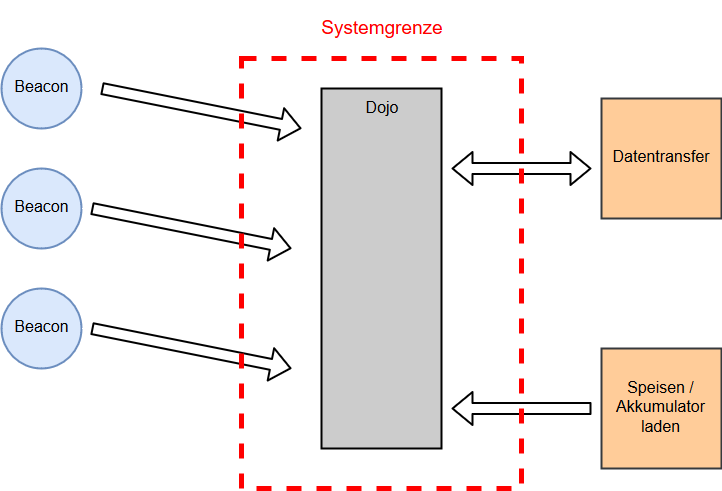
\includegraphics[width=140mm]{data/Loesungskonzept_Systemgrenzen.png}
	\caption{Systemgrenzen des Dojo} %picture caption
	\label{fig:first_layer}
\end{center}
\end{figure}

\subsection{Funktionen}
Die Funktionen sind in zwei Bereiche unterteilt. Einerseits sind die Funktionen für die Museumsbesucher beschrieben, welche nachfolgend als Nutzer bezeichnet werden. Zum anderen die für die Museumsbetreiber relevanten Funktionen. Diese werden nachfolgend als Betreiber bezeichnet.
\subsubsection*{Nutzer}
Der Nutzer geht mit dem Dojo durch das Museum. Sobald die Bluetooth Beacons genug nahe sind, wird dem Nutzer ein Signal gesendet. Dies erfolgt durch Vibration oder mithilfe einer LED. Jetzt soll der Nutzer entscheiden ob er sich das zugehörige Audio-File anhören will. Will er das, kann er den Play-Button betätigen. Die Lautstärke kann über die Buttons justiert werden. Falls das Ausstellungsstück dem Nutzer gefallen hat, kann er die Merken-Taste betätigen. Diese speichert das Ausstellungsstück auf eine Liste im Dojo. Am Ende des Museumsbesuches kann diese Liste ausgewertet werden. Dies fällt aber nicht mehr in die zuvor definierten Systemgrenzen. Wir stellen nur sicher, dass die Liste exportiert werden kann.
\subsubsection*{Betreiber}
Der Betreiber muss den Dojo konfigurieren. Dies erfolgt über eine SD-Karte, welche mit dem Computer beladen wird. Anschliessend wird diese in den Dojo eingeführt. Das Nachladen des Akkumulator erfolgt über eine induktive Ladung. Die nächsten zwei Funktionen sind Wunschziele, die vor allem mit Rücksicht auf die Laufzeit realisiert werden. Den Bluetooth-Reciver könnte man kurzzeitig auf ein Bluetooth Beacon umschalten. Der Betreiber müsste nur noch einen Reciver pro Raum installieren. Damit könnte man die gewünschte HeatMap realisieren. Das zweite wäre die Möglichkeit per Bluetooth einzelne Audiofiles auf den Dojo zu übertragen, um im Falle einer Änderung der Austellung die Liste anzupassen.

\subsection{Teilsysteme}
Das Herzstück des Dojo ist ein NRF52 von Nordic Semiconductor mit integriertem Bluetooth-Stack, welcher wiederum low-Energy fähig ist. Die Daten werden auf einer SD-Karte gespeichert. Der NRF52 wird die Audiodaten an den Verstärker weitergeben, welcher sie über den Körperschallaktor ausgibt. Gespeist wird der Dojo von einem Akku, welcher induktiv geladen wird. Diese Teilsysteme werden in den nachfolgenden Kapiteln noch genauer erläutert.

\begin{figure}[H]
\begin{center}
	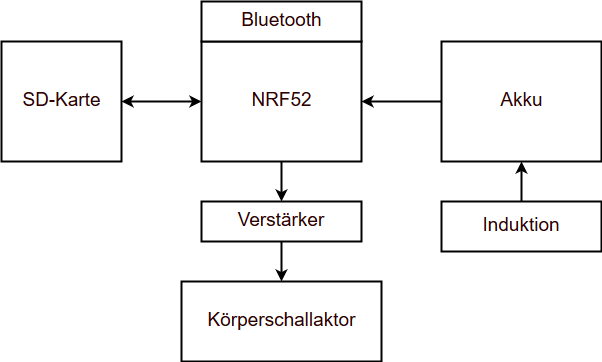
\includegraphics[width=120mm]{data/Loesungskonzept_Teilsysteme.png}
	\caption{Teilsysteme des Dojo} %picture caption
	\label{fig:first_layer}
\end{center}
\end{figure}


\subsection{Alternativer Ansatz}
Im unterstehenden Bild wird der alternative Ansatz gezeigt. Es gibt mehrere Gründe die gegen diesen Ansatz sprechen.
\begin{itemize}
\item Der Mux ist schwierig zu realisieren
\item Die SD-Karte über USB zu beladen ist anspruchsvoll
\item Auf den meisten Bluetooth-Modulen(HM-10) ist ein ähnlicher Chip verbaut wie der NRF52
\item Induktives Laden ist spannender als mit USB
\end{itemize}
Diese Gründe und das Gespräch mit Herr Gysin haben uns dazu veranlasst diese Variante zu verwerfen.

\begin{figure}[H]
\begin{center}
	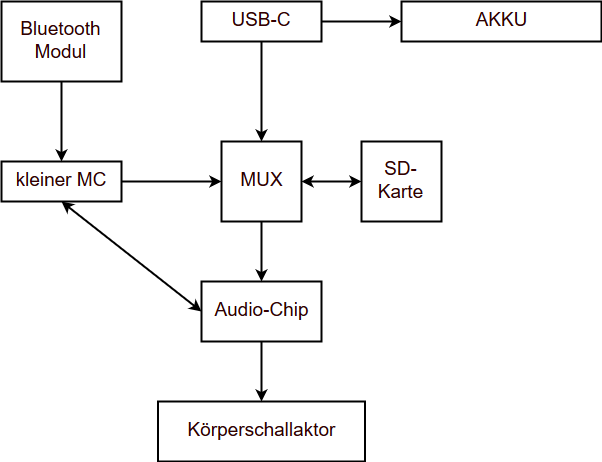
\includegraphics[width=120mm]{data/Loesungskonzept_alternativ.png}
	\caption{Alternatives Lösungskonzept} %picture caption
	\label{fig:first_layer}
\end{center}
\end{figure}


